\chapter{Desarrollo del entorno base}\label{ch:desarrollo-del-entorno-base}

En este capítulo se abordará el desarrollo de la aplicación base, empezando por la investigación
de tecnologías.
También se definirá la estructura final de la aplicación en los ámbitos de la interfaz y el código.


\section{Definición de los requisitos de las tecnologías candidatas}
\label{sec:definicion-requisitos-tecnologías-candidatas}

Actualmente, existe una gran variedad de librerías y \textit{frameworks} gráficos que permiten
crear aplicaciones de una manera rápida y sencilla.
Estas tecnologías se pueden clasificar dependiendo de una gran cantidad de criterios.

\noindent Según su nivel de abstracción:
\begin{itemize}
    \item \textbf{Librerías de bajo nivel:} son más cercanas al \textit{hardware} gráfico.
    Permiten tener un gran control sobre los gráficos, pero no son adecuadas para
    interfaces gráficas de usuarios.
    Algunos ejemplos de librerías de bajo nivel son \textit{OpenGL}, \textit{Vulkan} o \textit{DirectX}.
    \item \textbf{Librerías de alto nivel}: incorporan una capa de abstracción sobre el \textit{hardware} gráfico.
    Permiten generar interfaces gráficas de usuario mediante una arquitectura ya definida.
    Algunos ejemplos de librerías de alto nivel son \textit{Qt}, \textit{JavaFX}, \textit{Swing}, \textit{GTK} o
    \textit{Compose Multiplatform}.
\end{itemize}

\noindent Según su disponibilidad en varias plataformas:
\begin{itemize}
    \item \textbf{Librerías exclusivas:} son librerías que solo están disponibles en una plataforma.
    Algunos ejemplos de librerías exclusivas son \textit{Windows Forms} y \textit{DirectX} en \textit{Windows},
    \textit{Metal} y \textit{QuickDraw} en \textit{MacOS} o \textit{AndroidX/Graphics} y \textit{Jetpack Compose}
    en \textit{Android}.
    \item \textbf{Librerías multiplataforma:} están disponibles en una gran variedad de plataformas.
    Algunos ejemplos de librerías multiplataforma son \textit{Qt}, \textit{JavaFX}, \textit{Swing}, \textit{GTK}
    o \textit{Compose Multiplatform}.
\end{itemize}

\noindent Un aspecto muy importante al elegir candidatos es el \textbf{lenguaje de programación}
en el que las librerías están disponibles.
Las librerías de bajo nivel suelen estar disponibles en una gran variedad de lenguajes, mientras que las
librerías de alto nivel suelen incorporar paradigmas propios del lenguaje de programación en el que están
desarrolladas.

\noindent Para el desarrollo de la aplicación se desea utilizar una librería gráfica \textbf{moderna},
\textbf{de alto nivel} y \textbf{multiplataforma}, disponible en un lenguaje de programación estable,
con una comunidad grande y \textbf{rápido tanto en el desarrollo como en la ejecución}.
Otro requisito crucial es que el lenguaje permita \textbf{vincular código externo} de manera
sencilla.

\noindent Estos requisitos reduce la lista de tecnologías en los siguientes candidatos:
\begin{itemize}
    \item \textbf{HTML, CSS y TypeScript:} este conjunto de tecnologías es muy popular actualmente
    para la creación de aplicaciones web y de escritorio. \textit{IDEs} muy famosos como
    \textit{Visual Studio Code} están desarrollados con estas tecnologías.
    \item \textbf{Kotlin / Compose Multiplatform:} \textit{Compose Multiplatform} es una librería gráfica
    para \textit{Kotlin}, un lenguaje de programación muy joven y potente que tiene el respaldo de
    grandes compañías como \textit{JetBrains} y \textit{Google}.
    \item \textbf{Java / JavaFX:} \textit{JavaFX} puede considerarse la evolución natural de \textit{Swing},
    la herramienta principal para el desarrollo de aplicaciones gráficas basadas en \textit{Java}.
    \textit{JavaFX} es una librería moderna y rápida que, gracias a que está desarrollada en \textit{Java},
    puede ser empleada por otros lenguajes de programación que corren sobre la \textit{JVM}
    \footnote{\textit{Java Virtual Machine}}, como es el caso de \textit{Scala}, \textit{Groovy} o el ya mencionado
    \textit{Kotlin}.
\end{itemize}

\noindent El trío \textit{HTML / CSS / TypeScript} suele ser una buena elección para editores y otras
aplicaciones ligeras, pero la falta de velocidad en la ejecución y la falta de consistencia por estar
basado \textit{TypeScript} en \textit{JavaScript} descarta esta opción por parte del simulador.

\noindent \textit{Kotlin / Compose Multiplatform} es una elección muy sólida actualmente, pero esta
tecnología seguía en fase \textit{beta} cuando este proyecto empezó, por lo que también ha quedado
descartada.

\noindent Finalmente, \textbf{se ha optado por utilizar el par de tecnologías \textit{Java / JavaFX}}
para el desarrollo de la aplicación, ya que cumple con todos los requisitos: \textit{Java} es un
lenguaje de programación muy estable, multiplataforma y rápido tanto en la ejecución como en
el desarrollo.
También es el lenguaje de programación con la comunidad de desarrolladores más grande.
\textit{JavaFX} es una alternativa moderna a \textit{Swing} que permite desarrollar aplicaciones
fácilmente personalizables que se alejan del ya conocido estilo de interfaz \textit{Java}.

\noindent Centrándose en otras tecnologías necesarias, se ha utilizado el entorno de desarrollo
\textit{Intellij IDEA} y el sistema de automatización \textit{Gradle} para la construcción
del proyecto.

\subsection{En defensa de \textit{Java}}\label{subsec:en-defensa-de-java}

Muchos desarrolladores piensan que \textit{Java} es un lenguaje de programación verboso, lento, pesado
y con el único propósito de crear aplicaciones \textit{Spring}.
Que la mayoría de aplicaciones \textit{Java} estén desarrolladas en versiones \textit{vanilla}
\footnote{Estándar, sin modificar} de \textit{Swing} y en versiones de \textit{Java} de hace más
de un lustro no ayuda en su reputación.

\noindent La realidad es muy diferente: su equipo de desarrollo lleva años reinventando su tecnología,
con nuevas características que acercan a \textit{Java} a lenguajes de programación mucho más modernos.
La velocidad de ejecución también se ha incrementado considerablemente, posicionándose en uno de los
lenguajes de programación que más rápido ejecutan.

\noindent Un gran ejemplo del drástico cambio que ha sufrido \textit{Java} en los últimos años son los
\textit{records}: clases de datos que son inmutables.

\begin{lstlisting}[language=Java,style=java,frame=single,label={lst:java-comparacion-18}]
public record Cat(String name, UUID owner) {
}
\end{lstlisting}

\noindent El código equivalente en \textit{Java} 8 sería el siguiente:

\begin{lstlisting}[language=Java,style=java,frame=single,label={lst:java-comparacion-8}]
public final class Cat {
    private final String name;
    private final UUID owner;

    public Cat(String name, UUID owner) {
        this.name = name;
        this.owner = owner;
    }

    public String name() { return name; }

    public UUID owner() { return owner; }

    @Override
    public boolean equals(Object obj) {
        if (obj == this) return true;
        if (obj == null || obj.getClass() != this.getClass()) return false;
        var that = (Cat) obj;
        return Objects.equals(this.name, that.name) &&
                Objects.equals(this.owner, that.owner);
    }

    @Override
    public int hashCode() { return Objects.hash(name, owner); }

    @Override
    public String toString() { return "Cat[" + "name=" + name
        + ", " + "owner=" + owner + ']'; }

}
\end{lstlisting}

\noindent La nueva arquitectura basada en módulos que presenta las librerías de \textit{Java}
ayuda mucho en la distribución de aplicaciones de escritorio, pudiendo generar un instalador
convencional que instala la aplicación junto con una versión local de la \textit{JVM} que no
suele superar los 30 MB\cite{JPACKAGE}.
Gracias a este sistema de distribución, la aplicación podrá contar con versiones
de \textit{Java} actuales sin que los usuarios tengan que pasar por complejas instalaciones.

\noindent Como dato final, existen muchas aplicaciones que se ejecutan sobre la \textit{JVM}
sin que el usuario se de cuenta.
Este es el caso de todos los \textit{IDEs} desarrollados por \textit{JetBrains}, los cuales
usan la librería \textit{Swing} con un estilo avanzado.

\begin{figure}[H]
    \centering
    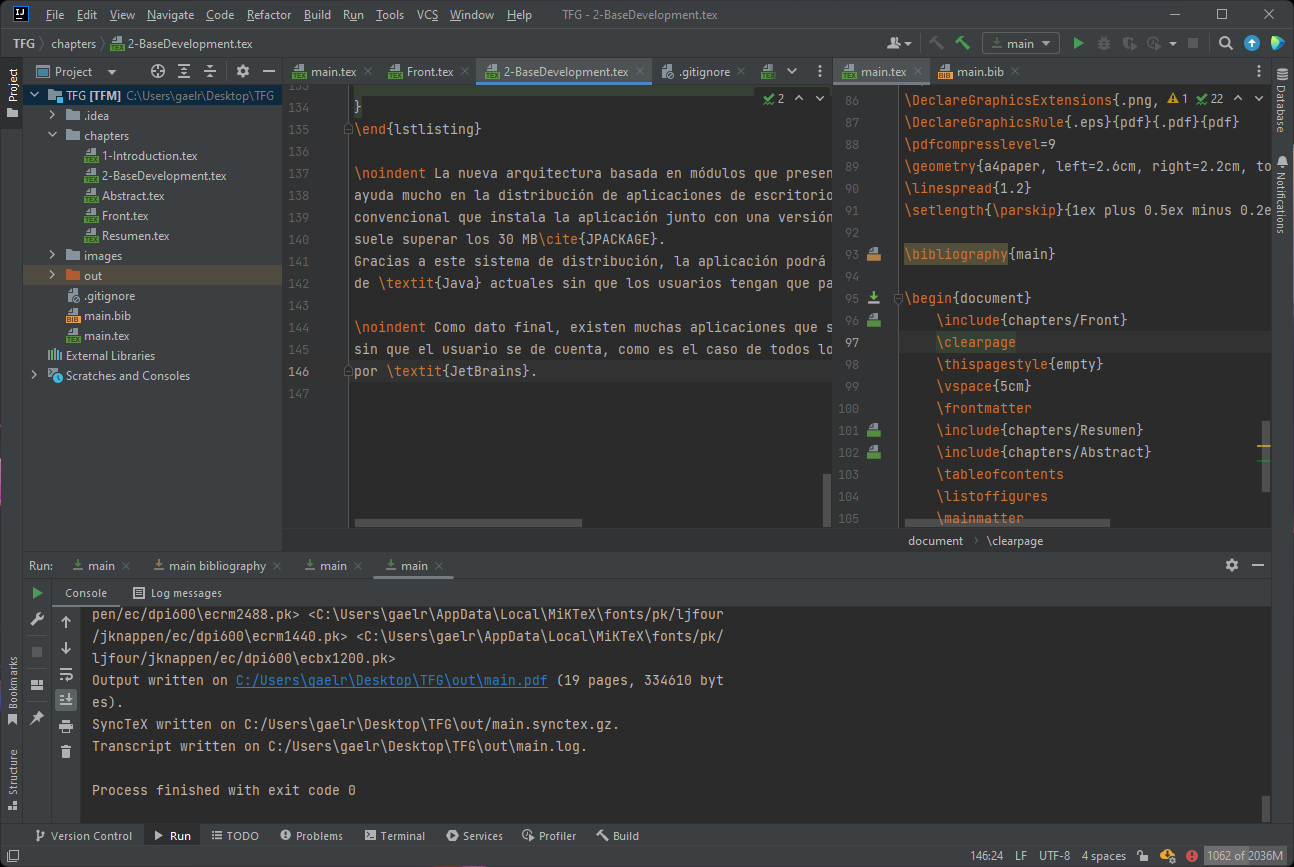
\includegraphics[width=\textwidth]{images/base/intellij-idea}
    \caption{\textit{Intellij IDEA}}
    \label{fig:java-intellij-idea}
\end{figure}


\section{Estructura del proyecto}\label{sec:estructura-del-proyecto}

\textit{JAMS} sigue los estándares de estructura de \textit{Gradle}\cite{GRADLE_ORGANIZING}.
Esto hace que su estructura sea muy similar a otras aplicaciones que usan el mismo
sistema de automatización.

\subsection{Tareas}\label{subsec:tareas}

\noindent El elemento más importante del directorio raíz es el archivo \textbf{build.gradle}.
En él se especifican las dependencias y se define cómo el proyecto debe ser compilado.
Las \textbf{tareas} son las encargadas de definir dicho comportamiento.

\noindent Las dos tareas más importantes son las siguientes:
\begin{itemize}
    \item \textbf{jpackage:} permite generar un instalador de la aplicación específico
    para la máquina que ejecuta la tarea.
    \item \textbf{bundle:} genera un archivo \textit{jar} con la aplicación y todas
    sus dependencias.
    Este archivo puede ser ejecutado en cualquier sistema operativo que pueda correr
    \textit{Java} y esté soportado por \textit{JavaFX}.
\end{itemize}

\noindent Para ejecutar estas tareas ha de usarse el \textit{script} \textbf{gradlew}.
Este comando descargará \textit{Gradle} si es necesario y ejecutará
la tarea pasada como argumento.
Todos estos comportamientos están automatizados en \textit{GitHub}
mediante los \textit{scripts} dentro de la carpeta \textbf{.github}.

\subsection{Módulos y paquetes}\label{subsec:modulos-y-paquetes}

Dentro de la carpeta \textbf{src} están definidos los dos módulos principales del
proyecto: \textbf{main} y \textbf{test}.

\noindent El módulo \textbf{main} es el encargado de almacenar todo el código fuente
de la aplicación.
Puede ser considerado el módulo más importante de todo el proyecto.
El módulo \textbf{test} define todas las pruebas unitarias que el módulo \textbf{main}
debe superar para que la aplicación se compile con éxito.

\noindent El código fuente almacenado en el módulo \textbf{main} está separado en diferentes
paquetes \textit{Java}:
\begin{itemize}
    \item \textbf{collection:} contiene una serie de colecciones modificadas.
    \item \textbf{configuration:} contiene el sistema de configuraciones.
    \item \textbf{event:} contiene el sistema de eventos.
    \item \textbf{file:} contiene los tipos de archivo definidos en la aplicación.
    \item \textbf{gui:} contiene toda la interfaz de la aplicación.
    \item \textbf{language:} contiene el sistema de idiomas.
    \item \textbf{manager:} contiene el sistema de gestores.
    \item \textbf{mips:} contiene todas las herramientas relacionadas con la arquitectura \textit{MIPS32}.
    \item \textbf{plugin:} contiene el sistema de componentes.
    \item \textbf{project:} contiene el sistema de proyectos.
    \item \textbf{task:} contiene el sistema de hijos y tareas asíncronas.
    \item \textbf{utils:} contiene clases útiles utilizadas por los anteriores paquetes.
\end{itemize}


\section{Proyectos}\label{sec:interfaz-grafica}

\textit{JAMS} es un \textit{IDE} basado en \textbf{proyectos}.
Un proyecto está formado por una carpeta y las siguientes propiedades:
\begin{itemize}
    \item \textbf{Tipo de proyecto:} especifica el tipo de proyecto.
    En una versión sin componentes este valor solo puede tomar el valor \textit{MIPS}.
    \item \textbf{Propiedades del proyecto:} parámetros necesarios por el tipo de proyecto.
    Configuran aspectos concretos y generales de todo el proyecto.
    \item \textbf{Archivos a ensamblar:} lista de archivos que el ensamblador tendrá en cuenta
    al ensamblar el proyecto.
    \item \textbf{Configuraciones:} especifican propiedades \textbf{de una ejecución} del proyecto.
    Es decir, configuran el simulador.
    Un proyecto puede tener varias configuraciones, y el usuario ha de elegir una al crear una
    simulación.
\end{itemize}

\noindent Los proyectos son almacenados en carpetas.
Una carpeta de un proyecto tiene la siguiente estructura:

\begin{center}
    \basictree{
        [MyProject
        [.jams
        [data.json]
        [files\_to\_assemble.json]
        ]
        [Simulation Files
        [MySimulationFile.txt]
        ]
        [MyAsmFile.asm]
        ]
    }
\end{center}

\noindent Cada proyecto tiene dos carpetas por defecto: \textbf{.jams} y
\textbf{Simulation Files}.
La carpeta \textbf{.jams} contiene los datos del proyecto que \textit{JAMS}
gestiona de manera automática.
Esta carpeta está oculta y no debe ser modificada por el usuario.
El archivo \textbf{data.json} contiene el tipo de proyecto y sus propiedades,
mientras que \textit{files\_to\_assemble.json} contiene la listas de archivos
que el ensamblador ha de usar.
La carpeta \textit{Simulation Files} actúa de carpeta raíz del simulador:
todos los archivos que escriba o lea el simulador deben estar situados dentro
de esta carpeta.


\section{Gestores}\label{sec:gestores}

Toda la arquitectura de la aplicación está basada en \textbf{gestores}.
Un gestor se puede definir como un conjunto de elementos que las herramientas pueden usar.
\textit{JAMS} proporciona tres tipos básicos de gestores:
\begin{itemize}
    \item \textbf{Gestores normales:} implementados por la clase \textit{Manager}.
    Contienen una lista de elementos sin ninguna jerarquía.
    \item \textbf{Gestores con valor por defecto:} actúa como un gestor normal, con la
    diferencia que uno de sus valores es el valor por defecto.
    Estos gestores heredan de la clase \textit{DefaultValuableManager}.
    \item \textbf{Gestores con valor seleccionado:} actúan como un gestor con valor por defecto,
    pero con uno de los elementos seleccionado.
    Cuando el elemento seleccionado se elimina, el elemento por defecto queda seleccionado.
    Estos gestores heredan de la clase \textit{SelectableManager}.
\end{itemize}

\subsection{Proveedores}\label{subsec:proveedores}

Cada elemento guardado en un gestor \textbf{está asociado al proveedor que lo proporciona}.
Un proveedor puede ser un plugin o el propio \textit{JAMS}.
Cuando un proveedor se desvincula de la aplicación, todos los elementos proporcionados
por el proveedor son eliminados de los gestores.

\subsection{Registro}\label{subsec:registro}

El registro es un \textbf{elemento estático dentro de la aplicación}.
Se puede considerar un \textbf{gestor de gestores}.
En el registro se pueden recuperar, añadir, eliminar o modificar gestores.
Igual que los gestores normales, cuando un proveedor se desvincula de la aplicación,
todos los gestores proporcionados por el proveedor son eliminados del registro.

\noindent \textit{JAMS} permite separar los gestores en dos tipos:
\textbf{gestores primarios} y \textbf{gestores secundarios}.
Los gestores primarios son fácilmente accesibles cuando se busca un gestor por tipo
usando métodos como \textbf{Manager.of(Type.class)}.
Solo puede existir un gestor primario por tipo.
Para buscar gestores secundarios, se debe proveer el nombre del gestor explícitamente.

\subsection{Acceder a los gestores}\label{subsec:acceder-a-los-gestores}

Existen dos maneras de acceder a un gestor: \textbf{usando el registro} o
\textbf{usando los atajos de la clase Manager}.

\begin{lstlisting}[language=Java,style=java,frame=single,label={lst:acceder-a-los-gestores}]
// Returns the primary manager that manages languages.
Manager<Language> simpleLanguageManager = Manager.of(Language.class);
simpleLanguageManager = Jams.REGISTRY.of(Language.class);

// Returns the primary selectable manager that manages languages.
SelectableManager<Language> selectableLanguageManager = Manager.ofS(Language.class);
selectableLanguageManager = (SelectableManager<Language>) Jams.REGISTRY.of(Language.class);

// Returns the manager that is an instance of LanguageManager.
LanguageManager languageManager = Manager.get(LanguageManager.class);
languageManager = Jams.REGISTRY.get(LanguageManager.class);

// Returns the manager with the given name.
Manager<Language> manager = Jams.REGISTRY.of("other-language-manager", Language.class);
\end{lstlisting}

\subsection{Usar los gestores}\label{subsec:usar-los-gestores}

Los \textbf{gestores} implementan la interfaz \textbf{Set}
\footnote{https://docs.oracle.com/javase/8/docs/api/java/util/Set.html},
por lo que son fácilmente manipulables.

\begin{lstlisting}[language=Java,style=java,frame=single,label={lst:usar-los-gestores}]
SelectableManager<Language> manager = Manager.ofS(Language.class);

// Accessing elements
Language selectedLanguage = manager.getSelected();
Optional<Language> english = manager.get("English");

// Iterate through the manager
manager.forEach(language -> System.out.println(language.getName()));

// Adding and removing elements
if (english.isPresent()) {
    manager.remove(english.get());
    manager.add(english.get());
}
\end{lstlisting}

\subsection{Crear nuevos gestores}\label{subsec:crear-nuevos-gestores}

Se pueden crear gestores de cualquier tipo de dato que extienda la interfaz \textbf{ManagerResource}.

\begin{lstlisting}[language=Java,style=java,frame=single,label={lst:crear-nuevos-gestores}]
// The element to store inside the manager
public record MyElement(ResourceProvider provider, String name, double value) implements ManagerResource {
    @Override
    public ResourceProvider getResourceProvider() {return provider;}

    @Override
    public String getName() {return name;}
}

// The manager implementation
public class MyManager extends Manager<MyElement> {

    public MyManager(ResourceProvider provider) {
        super(provider, "my-manager", MyElement.class, false);
    }

    @Override
    protected void loadDefaultElements() {
        add(new MyElement(provider, "test-1", 1.0));
        add(new MyElement(provider, "test-2", 2.0));
        add(new MyElement(provider, "test-3", 3.0));
    }
}
\end{lstlisting}


\section{Eventos}\label{sec:eventos}

\textit{JAMS} incluye un sistema de eventos que permite informar de sucesos entre componentes de la aplicación.
Este sistema está profundamente inspirado en el sistema de eventos usado por la comunidad de \textit{Minecraft}
en proyectos como \textit{Spigot}\footnote{https://www.spigotmc.org/}
o \textit{Sponge}\footnote{https://www.spongepowered.org/}, y puede considerarse una evolución descentralizada
de esta tecnología.

\subsection{Emisores de eventos}\label{subsec:emisores-de-eventos}

Los emisores de eventos son los encargados de relacionar los creadores de eventos con sus escuchadores.
Un emisor de evento está representado por la interfaz \textbf{EventBroadcast}.
Esta interfaz es implementada por cualquier elemento que quiera ser usado para registrar escuchas.
Los gestores, los componentes, o el propio \textit{JAMS} implementan un emisor por defecto.
La clase \textbf{SimpleEventBroadcast} contiene una implementación de \textbf{EventBroadcast}
que se puede usar como superclase.

\subsection{Definir escuchas}\label{subsec:definir-escuchas}

Las escuchas son \textbf{métodos no estáticos anotados con la anotación @Listener}.
Estos métodos solo tienen un parámetro que pide un elemento que extienda la clase
\textbf{Event} y deben devolver \textbf{void}.

\begin{lstlisting}[language=Java,style=java,frame=single,label={lst:definir-escuchas}]
@Listener
private void onLanguageRegister(ManagerElementRegisterEvent.After<Language> event) {
    System.out.println("New language available! " + event.getElement().getName());
}
\end{lstlisting}

\noindent Este método, después de ser registrado en un gestor de idiomas,
se ejecutará cuando un nuevo idioma sea añadido al gestor.

\noindent A diferencia de otros sistemas de eventos similares,
el sistema de eventos de \textit{JAMS} permite usar \textbf{eventos genéricos}.
Un ejemplo es el caso anterior, donde el método pide un elemento de tipo
\textbf{ManagerElementRegisterEvent.After<Language>}.
Si el emisor al que está registrado emite un evento de tipo
\textbf{ManagerElementRegisterEvent.After<Theme>}, la escucha no será invocada.

\noindent Un evento puede extender la clase de otro evento.
Esto permite generar una jerarquía de eventos.
Una escucha que pide un cierto tipo de evento se ejecutará siempre que dicho evento o uno de sus hijos ocurra.
Si una escucha pide el evento \textbf{Event}, su método se ejecutará siempre que un evento ocurra.

\noindent Algunos eventos implementan la interfaz \textbf{Cancellable}, lo cual permite cancelar el evento.
Las escuchas restantes no serán llamadas cuando un evento es cancelado salvo que se defina lo contrario
en la etiqueta \textbf{@Listener}.

\subsection{Registrar escuchas}\label{subsec:registrar-escuchas}

Una vez se tenga una escucha definida, esta se puede registrar en uno o varios emisores de eventos.
Al ser las escuchas no estáticas, toda escucha registrada en un emisor está ligada al evento con el
que debe ser invocado.
Esto añade una gran flexibilidad al sistema, permitiendo que un elemento registre
escuchas dependiendo de su estado.

\noindent El método más usado para registrar escuchas es el método
\textbf{registerListeners(Object, boolean)}.
Este método buscará en el objeto todos los métodos con la etiqueta \textbf{@Listener}
que pidan un evento y devuelvan \textbf{void}.
Esta búsqueda incluye a todos los métodos definidos en el objeto,
incluyendo métodos privados y métodos de las superclases.

\noindent El booleano \textbf{useWeakReferences} permite registrar la escucha usando una referencia débil.
Si este booleano es falso, el objeto usado para el registro quedará en memoria aunque todas
sus referencias cesen de existir, por lo que se debe eliminar el registro de manera manual.
La referencia débil elimina este paso, borrándose el registro automáticamente cuando
el elemento deja de ser referenciado.

\begin{lstlisting}[language=Java,style=java,frame=single,label={lst:registrar-escuchas}]
private void register() {
    Manager<Language> manager = Manager.of(Language.class);
    manager.registerListeners(this, true);
}

@Listener
private void onLanguageRegister(ManagerElementRegisterEvent.After<Language> event) {
    System.out.println("New language available! " + event.getElement().getName());
}
\end{lstlisting}

\noindent Si se desea, se puede registrar una única escucha del objeto.
Este método requiere conocimientos de la librería \textit{reflection} de \textit{Java}:

\begin{lstlisting}[language=Java,style=java,frame=single,label={lst:registrar-escuchas-2}]
private void register() throws NoSuchMethodException {
    Manager<Language> manager = Manager.of(Language.class);
    manager.registerListener(
            this,
            this.getClass().getDeclaredMethod("onLanguageRegister", ManagerElementRegisterEvent.class),
            true
    );
}

@Listener()
private void onLanguageRegister(ManagerElementRegisterEvent.After<Language> event) {
    System.out.println("New language available! " + event.getElement().getName());
}
\end{lstlisting}

\noindent Para eliminar los registros, se han de usar los métodos análogos
\textbf{unregisterListeners} y \textbf{unregisterListener}.

\subsection{Parámetros avanzados}\label{subsec:parámetros-avanzados}

La etiqueta \textbf{@Listener} permite definir comportamientos más avanzados en la escucha.

\begin{lstlisting}[language=Java,style=java,frame=single,label={lst:escuchas-avanzadas}]
@Listener(priority = 20, ignoreCancelled = true)
private void onLanguageRegister(ManagerElementRegisterEvent.After<Language> event) {
    System.out.println("New language available! " + event.getElement().getName());
}
\end{lstlisting}

\noindent El parámetro \textbf{priority} permite definir la prioridad de la escucha.
La escucha con el número más alto será la primera en ser llamada.
El parámetro \textbf{ignoreCancelled} es un booleano que le da a la escucha la capacidad
de ser llamada incluso cuando un evento ha sido cancelado.


\section{Interfaz de usuario}\label{sec:interfaz-de-usuario}

La interfaz de \textit{JAMS} es muy similar a las interfaces que presentan los \textit{IDEs} modernos.
Todas las herramientas están encapsuladas en \textbf{nodos}.
Cada nodo se puede desplegar en los laterales del editor.
Más concretamente, se pueden desplegar dos nodos por cada lado del editor.

\begin{figure}[H]
    \centering
    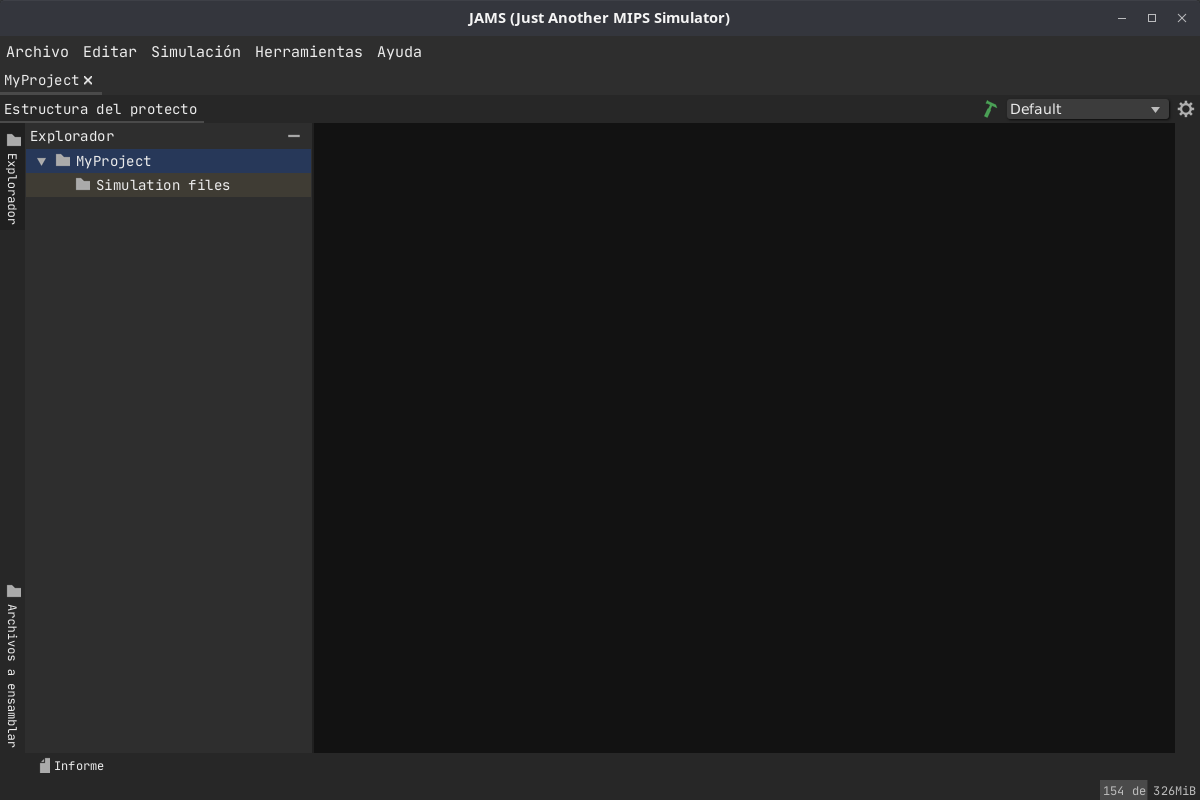
\includegraphics[width=0.8\textwidth]{images/base/jams-basic}
    \caption{\textit{Editor de \textit{JAMS} en su forma más básica}}
    \label{fig:jams-basic}
\end{figure}

\noindent Los nodos también se pueden configurar para que se desplieguen en una ventana aparte.
Esto permite poder desplegar un número indefinido de nodos al mismo tiempo.
El modo de despliegue se puede configurar presionando el botón secundario sobre
el botón del nodo.

\begin{figure}[H]
    \centering
    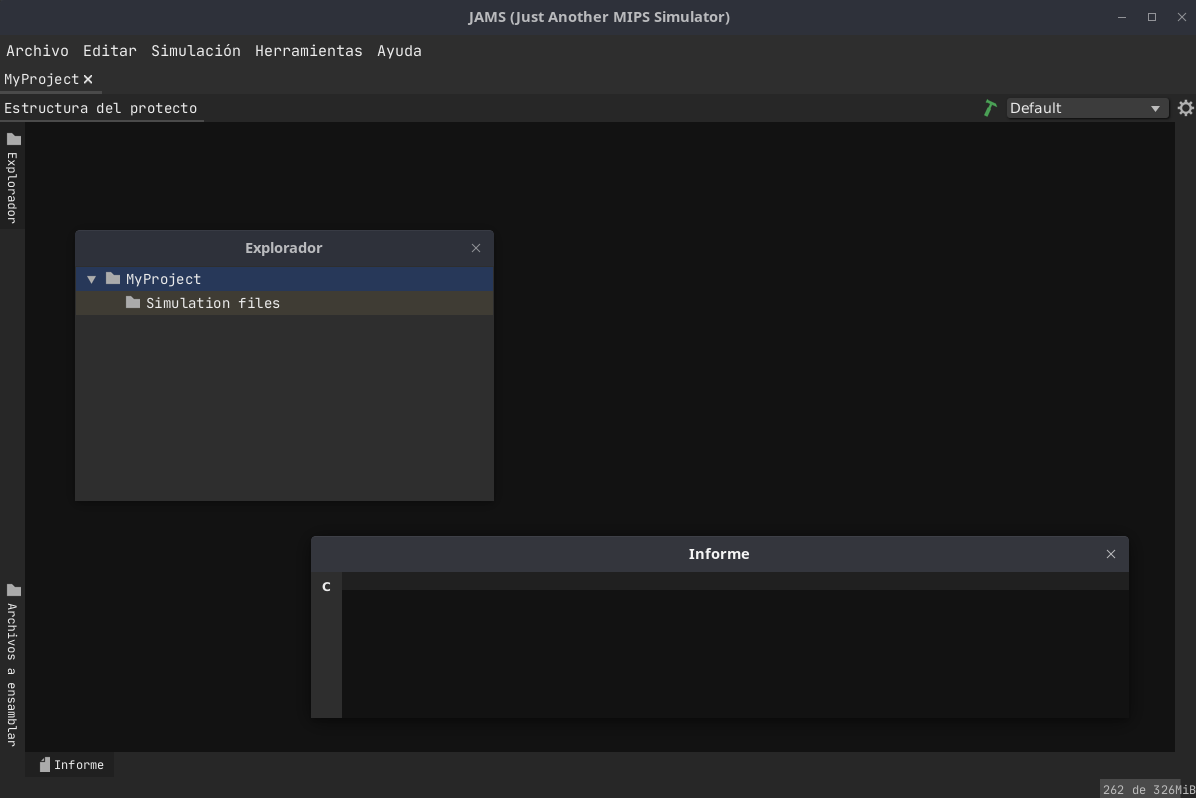
\includegraphics[width=0.8\textwidth]{images/base/jams-windows}
    \caption{\textit{Editor de \textit{JAMS} con ventanas desplegadas}}
    \label{fig:jams-windows}
\end{figure}

\subsection{Menú superior}\label{subsec:menu-superior}

El menú superior de \textit{JAMS} funciona de manera idéntica a cualquier otro programa.
Por defecto existen cinco secciones:
\begin{itemize}
    \item \textbf{Archivo}: permite crear o abrir nuevos proyectos, además de
    acceder a la configuración.
    \item \textbf{Editar:} permite acceder a los comandos del editor de texto.
    \item \textbf{Simulación:} permite acceder a los comandos de simulación.
    \item \textbf{Herramientas:} permite habilitar o deshabilitar nodos.
    \item \textbf{Ayuda:} permite acceder a ayuda sobre \textit{JAMS}.
\end{itemize}

\subsection{Proyectos abiertos}\label{subsec:proyectos-abiertos}

Los proyectos abiertos aparecen justo debajo del menú superior.
Cada proyecto está representado por una pestaña, lo que facilita alternar entre
proyectos abiertos.
Si se cierran todos los proyectos, \textit{JAMS} cerrará el editor y trasladará
al usuario a la ventana de inicio.

\noindent Los proyectos presentan una lista de pestañas con todas las secciones
que tienen abiertas.
Normalmente, la primera pestaña representa el editor del proyecto, mientras que
las siguientes representan las simulaciones que el usuario vaya creando.

\begin{figure}[H]
    \centering
    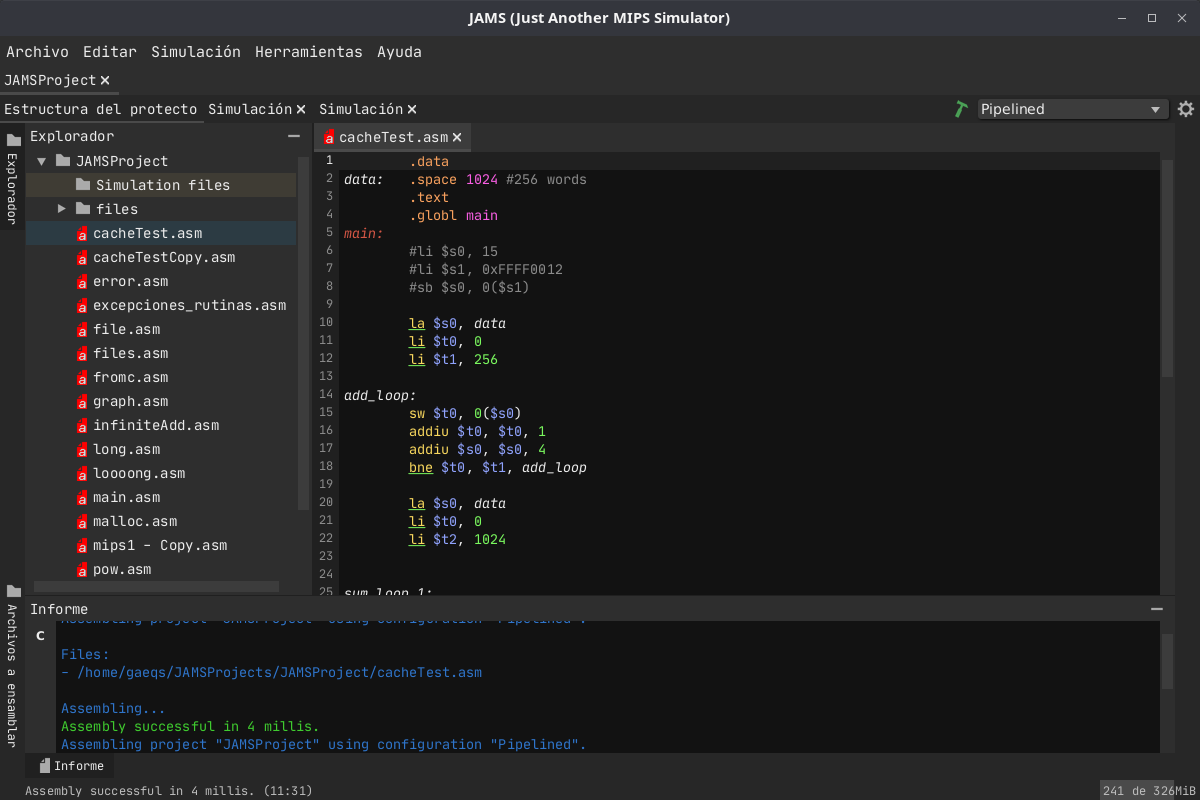
\includegraphics[width=0.8\textwidth]{images/base/jams-sections}
    \caption{\textit{Editor de \textit{JAMS} con varias simulaciones creadas}}
    \label{fig:jams-sections}
\end{figure}

\noindent Cada sección tiene una \textbf{barra de herramientas} propia.
Esta barra está situada a la izquierda de la lista de secciones, y permite
ejecutar acciones relacionadas con la sección actual.

\subsection{Barra inferior}\label{subsec:barra-inferior}

La barra inferior del editor es común a todas las secciones.
En esta, se informa del último mensaje escrito en el \textbf{informe}.
A la izquierda también se muestra la memoria que está usando actualmente
\textit{JAMS}.
Al estar creada la aplicación en \textit{Java}, esta utiliza un recolector
de basura.
Se puede forzar el paso del recolector de basura pulsando el panel que informa
sobre el uso de memoria.

\subsection{Ventana principal}\label{subsec:ventana-principal}

Si \textit{JAMS} no tiene ningún proyecto que mostrar, se mostrará la ventana
principal.
En esta ventana se pueden encontrar cuatro apartados:
\begin{itemize}
    \item \textbf{Proyectos:} en este apartado se encuentran los proyectos más
    recientes.
    También se puede abrir un proyecto ya existente.
    \item \textbf{Nuevo proyecto:} este apartado permite crear nuevos proyectos.
    Un componente puede añadir su propio creador de proyectos.
    \item \textbf{Configuración:} muestra la ventana de configuración.
    Permite configurar \textit{JAMS} antes de abrir un proyecto.
    \item \textbf{Acerca de:} muestra información básica sobre \textit{JAMS}.
\end{itemize}

\begin{figure}[H]
    \centering
    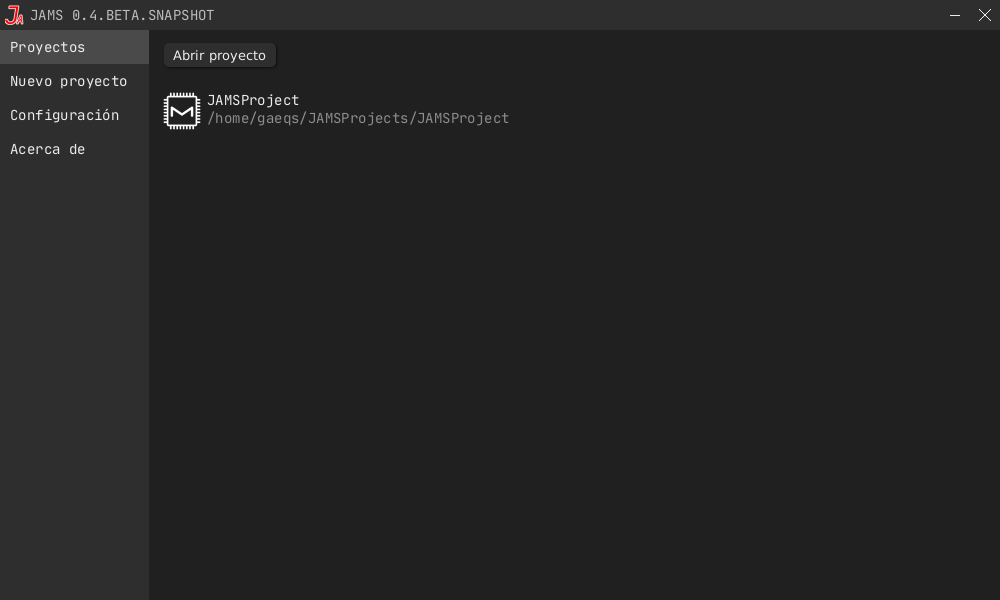
\includegraphics[width=0.8\textwidth]{images/base/jams-main-projects}
    \caption{\textit{Ventana principal mostrando los proyectos recientes}}
    \label{fig:jams-main-projects}
\end{figure}

\begin{figure}[H]
    \centering
    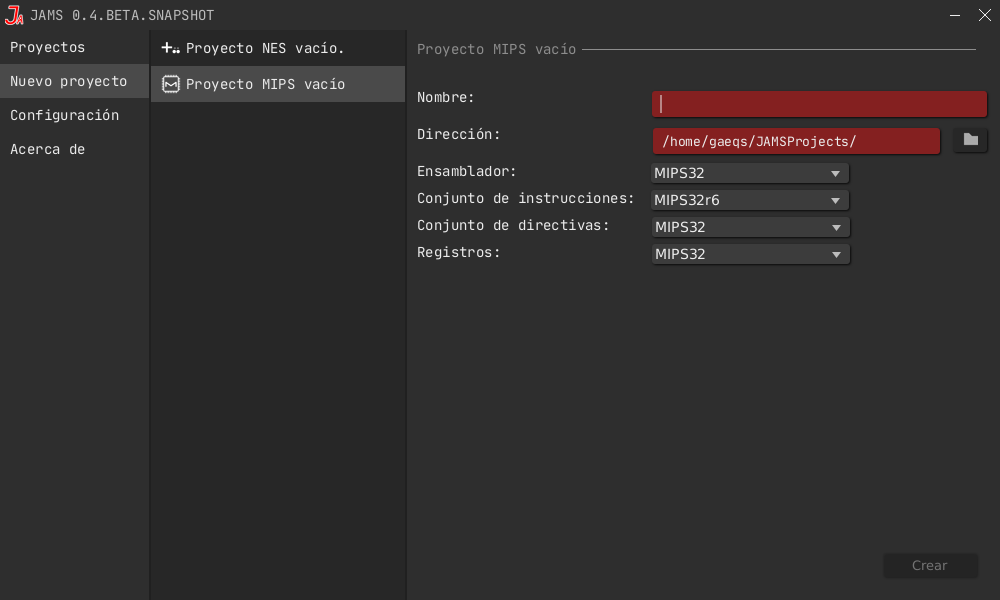
\includegraphics[width=0.8\textwidth]{images/base/jams-main-new-project}
    \caption{\textit{Ventana de creación de nuevos proyectos}}
    \label{fig:jams-main-new-project}
\end{figure}


\section{Idiomas}\label{sec:idiomas}

Igual que cualquier aplicación moderna, \textit{JAMS} presenta un sistema de
localización basado en paquetes de idiomas.
Cualquier usuario o componente puede crear un paquete que añada
o modifique un idioma.

\subsection{Estructura de un paquete}\label{subsec:estructura-de-un-paquete}

Un paquete de idiomas es una carpeta o un archivo comprimido
que contienen un archivo \textbf{language.json} y varios archivos \textit{YAML}.
Esta carpeta o archivo estará situado dentro de un componente
o dentro de la carpeta \textbf{~/JAMS/languages}.
Un ejemplo de un archivo \textbf{language.json} sería el siguiente:

\begin{lstlisting}[frame=single,label={lst:language.json}]
{
  "name": "English",
  "priority": 0,
  "files": [
    "actions.yml",
    "configuration.yml",
    "directives.yml",
    "editor.yml",
    "general.yml",
    "instructions.yml",
    "interface.yml",
    "mips_elements.yml",
    "mips_simulation_configuration.yml",
    "simulation.yml"
  ]
}
\end{lstlisting}

\noindent Dentro de este archivo se encuentran los siguientes parámetros:
\begin{itemize}
    \item \textbf{name:} es el nombre del idioma.
    Este nombre es el que será mostrado al usuario
    y actúa como identificador del idioma.
    \item \textbf{files:} son los archivos \textit{YAML} que componen el paquete.
    \item \textbf{priority:} es la prioridad del paquete si existen varios
    paquetes para el mismo idioma.
    Cuanto más alto sea el número, más prioridad tiene el paquete.
    Esta propiedad es opcional y por defecto toma el valor 0.
\end{itemize}

\noindent Los archivos \textit{YAML} pueden estar en carpetas dentro del paquete,
y deben estar definidos en el archivo \textbf{language.json} con una
dirección relativa a la raíz del paquete.
Un ejemplo de archivo \textit{YAML} sería el siguiente:

\begin{lstlisting}[frame=single,label={lst:interface.yml}]
START_TITLE: JAMS {VERSION}
START_PROJECTS: Projects
START_NEW_PROJECT: New project
START_ABOUT: About
BOTTOM_BAR_MEMORY: '{USED} of {TOTAL}MiB'
BOTTOM_BAR_MEMORY_TOOLTIP: Click to execute the garbage collector.

MAIN_MENU_FILE: File
MAIN_MENU_EDIT: Edit
MAIN_MENU_SIMULATION: Simulation
MAIN_MENU_TOOLS: Tools
MAIN_MENU_HELP: Help
MAIN_MENU_FILE_EXIT: Exit
MAIN_MENU_FILE_SETTINGS: Settings
MAIN_MENU_FILE_OPEN_PROJECT: Open project
MAIN_MENU_FILE_CREATE_PROJECT: Create project
MAIN_MENU_FILE_CREATE_PROJECT_TITLE: Create project
MAIN_MENU_FILE_CREATE_PROJECT_NAME: 'Name:'
MAIN_MENU_FILE_CREATE_PROJECT_PATH: 'Path:'
MAIN_MENU_HELP_ABOUT: About
\end{lstlisting}

\noindent Aunque no se use en ningún paquete por defecto,
los paquetes de idiomas permiten crear secciones como
en cualquier archivo \textit{YAML}.
En el siguiente caso, se usará el identificador
\textbf{ACTION.MY\_ACTION} para referenciar el mensaje.

\begin{lstlisting}[frame=single,label={lst:yaml-subsection}]
ACTION:
  MY_ACTION: My action
\end{lstlisting}

\subsection{Extensiones}\label{subsec:idiomas-extensiones}

Puede existir el caso donde varios paquetes hagan referencia al mismo idioma.
Este problema de colisión se soluciona gracias a las extensiones.
Un paquete actúa siempre como una extensión de un idioma.
Esta extensión tiene una prioridad que se define en el archivo
\textbf{language.json} del paquete.
Si dos extensiones tienen la misma prioridad, el orden se resuelve
por orden de creación de la extensión, siendo el último en ser creado
el que tenga más prioridad.
El mensaje ligado a un identificador será el de la extensión con más prioridad
que contenga un mensaje ligado al identificador.
Gracias a este pequeño sistema de extensiones, los usuarios podrán crear modificaciones
y los componentes podrán añadir nuevos mensajes.

\subsection{Acceder a mensajes}\label{subsec:acceder-a-mensajes}

Existen dos maneras de acceder a los mensajes mediante un identificador:
\textbf{de manera directa} o \textbf{usando un componente preparado}.

\noindent Un componente puede acceder al idioma seleccionado usando
el gestor de idiomas por defecto.
La manera más correcta para pedir un mensaje es usando el método
\textbf{getOrDefault(String)} del idioma.
Este método devolverá el mensaje asociado al identificador dado.
Si el idioma no contiene ningún mensaje con ese identificador,
lo buscará en el idioma por defecto.
Si ninguno de los dos idiomas contiene el mensaje,
devuelve una cadena de texto vacía.

\noindent Cabe destacar que esta acción suele deber rehacerse cuando
el idioma cambia, por lo que se debe registrar una escucha en el
gestor de idiomas, escuchando el evento \textbf{LanguageRefreshEvent}.
Si esto no se hace, el seguirá mostrando el mensaje en el idioma
anterior.

\begin{lstlisting}[language=Java,style=java,frame=single,label={lst:idioma-escucha}]
@Listener
public void onRefresh(LanguageRefreshEvent event) {
    refreshMessage(event.getSelectedLanguage());
}
\end{lstlisting}

\noindent También existe una gran variedad de nodos de \textit{JavaFX} preparados
para usar mensajes traducibles, sin necesidad de que el desarrollador tenga que
gestionar escuchas y gestores.
Estos nodos se pueden encontrar en el paquete
\textbf{net.jamsimulator.jams.language.wrapper}.

\begin{lstlisting}[language=Java,style=java,frame=single,label={lst:idioma-nodo}]
new LanguageLabel(Messages.ACTION_FOLDER_EXPLORER_ELEMENT_NEW_FOLDER)
\end{lstlisting}


\section{Temas}\label{sec:temas}

Los temas de JAMS funcionan de la misma manera que el estilo de una página web:
mediante archivos \textit{CSS}.
funcionamiento de los temas es muy similar al funcionamiento de los idiomas:
los temas son empaquetados en una carpeta o archivo comprimido,
con un archivo \textit{JSON} que actúa como punto de entrada (\textbf{theme.json})
y un conjunto de archivos \textit{CSS}.

\noindent A diferencia de los idiomas, un desarrollador que implemente nuevos
nodos a la escena de \textit{JAMS} no require gestionar ningún aspecto
de los temas: el tema que el usuario tenga seleccionado será implementado
de manera transparente gracias al sistema de temas de \textit{JavaFX}.

\subsection{Estructura}\label{subsec:estructura}

El archivo \textbf{theme.json} define el nombre y los archivos
\textit{CSS} incluidos en el tema.
Un ejemplo de archivo theme.json sería el siguiente:
\begin{lstlisting}[frame=single,label={lst:theme.json}]
{
  "name": "Light Theme",
  "dependencies": ["Other Theme"],
  "files": [
    "extra.css"
  ]
}
\end{lstlisting}

\noindent Un archivo \textbf{theme.json} presenta los siguientes parámetros:
\begin{itemize}
    \item \textbf{name:} es el nombre del tema.
    Este nombre es el que será mostrado al usuario
    y actúa como identificador del tema.
    \item \textbf{files:} son los archivos \textit{CSS} que componen el paquete.
    \item \textbf{dependencies:} los temas de los que este tema depende.
    El estilo de estos temas será añadido al estilo del tema definido.
    Este parámetro es opcional.
\end{itemize}

\noindent Estén definidos o no las dependencias,
todo tema depende del tema \textbf{Common}.
Este tema actúa de base, y define el estilo básico de \textit{JAMS}.
Este tema define muchas variables globales, pero no le asigna ningún
valor a ninguna de ellas.

\subsection{Variables globales}\label{subsec:variables-globales}

Las variables globales permiten definir el color de los diferentes
componentes de manera muy sencilla.
Un tema debe asignar un color a todas las variables del tema \textbf{Common}.
Esta tarea se debe hacer en el archivo especial \textbf{global.css}.
Este archivo es un archivo especial que siempre está incluido en el tema y,
al compilar, será envuelto en una sección global \textit{CSS} \textbf{*\{ \}}.
Esto permite que todos los componentes puedan usar
las variables asignadas en este archivo.
Un ejemplo de archivo \textbf{global.css} sería el siguiente:

\begin{lstlisting}[frame=single,label={lst:global.css}]
-theme-foreground: #222222;
-theme-foreground-darker: derive(-theme-foreground, 20%);
-theme-foreground-darker-2: derive(-theme-foreground, 40%);
-theme-foreground-lighter: #000000;
-theme-background: #f2f2f2;
-theme-background-darker: #e5e5e5;
-theme-background-darker-2: #eaeaea;
-theme-background-lighter: #f7f7f7;
-theme-background-pressed: derive(-theme-background, -10%);
-theme-background-darkest: #FFFFFF;
-theme-shadow: #555555;
-theme-header: #8faccc;
-theme-menu-item-hover: #4D6EAF;

...
\end{lstlisting}

\subsection{Extensiones}\label{subsec:temas-extensiones}

Igual que los idiomas, los temas funcionan mediante extensiones.
Todo paquete de temas es convertido en una extensión del tema que define.
Si existen varios paquetes apuntando al mismo tema, los dos coexistirán
como dos extensiones del mismo tema.
Una gran diferencia a los idiomas es que las extensiones de los temas
no tienen prioridad.
\textit{JavaFX} sigue el estándar
\textit{CSS}\footnote{\url{https://developer.mozilla.org/en-US/docs/Web/CSS/Specificity\#how_is_specificity_calculated}}
para la prioridad de las definiciones,
por lo que una capa de prioridades más es innecesaria.


\section{Configuración}\label{sec:configuracion}

Igual que cualquier aplicación moderna, \textit{JAMS} presenta una
ventana de configuración donde el usuario podrá personalizar su experiencia.
Internamente, el sistema de configuraciones orbita alrededor de dos archivos \textit{JSON}:
\textbf{el archivo de valores} y el \textbf{archivo de estructura}.

\noindent El archivo de valores es el encargado de almacenar los valores de
todos los \textbf{nodos} de la configuración.
Existe dos versiones de este archivo:
el primero se encuentra en la carpeta \textbf{~/JAMS} y representa los \textbf{valores
actuales de la configuración}.
El segundo se encuentra dentro de la propia aplicación, y es el encargado de
proporcionar \textbf{los valores por defecto de cada nodo}.
Un componente podrá agregar nuevos valores a este archivo.

\begin{lstlisting}[frame=single,label={lst:main_config.json}]
{
    "language": {
        "default": "English",
        "selected": "English"
    },
    "appearance": {
        "theme": "Dark Theme",
        "hide_top_bar": false,
        "general_font": "JetBrains Mono",
        "code_font": "JetBrains Mono",
        "antialiasing": true
    },
    "editor": {
        "zoom_using_mouse_wheel": true,
        "reset_zoom_using_middle_button": true,
        "zoom_sensibility": 0.007,
        "mips": {
            "use_tabs": true,
            "preserve_tabs": true,
            "preserve_tabs_before_labels": true,
            "space_after_instruction": "SPACE",
            "space_after_instruction_parameter": "COMMA_AND_SPACE",
            "space_after_directive": "SPACE",
            "space_after_directive_parameter": "SPACE",
            "maximum_blank_lines": 2
        }
    }
}
\end{lstlisting}

\noindent El archivo de estructura o metadatos contiene información
relacionada sobre el propio nodo: el \textbf{tipo}, \textbf{región}
y \textbf{nombre} de cada nodo están definidos en este archivo.
Las secciones también tienen sus propios metadatos, especificando
el \textbf{nombre} de la sección y sus \textbf{regiones} con sus
\textbf{prioridades}.

\begin{lstlisting}[frame=single,label={lst:main_config_meta.json}]
{
    "language": {
        "meta": {
            "language_node": "CONFIG_LANGUAGE",
            "regions": {
                "language": 0
            }
        },
        "default": {
            "type": "language",
            "language_node": "CONFIG_LANGUAGE_DEFAULT",
            "region": "language"
        },
        "selected": {
            "type": "language",
            "language_node": "CONFIG_LANGUAGE_SELECTED",
            "region": "language"
        }
    }
}
\end{lstlisting}

\subsection{Interfaz de la configuración}\label{subsec:interfaz-de-la-configuración}

Para evitar que los usuarios tengan que modificar los valores de la configuración
externamente, se ha implementado una interfaz que permite modificar los
parámetros al vuelo dentro de la aplicación.
Esta interfaz es accesible directamente en la ventana de inicio o accediendo a ella
mediante la opción \textbf{Archivo > Configuración}.

\begin{figure}[H]
    \centering
    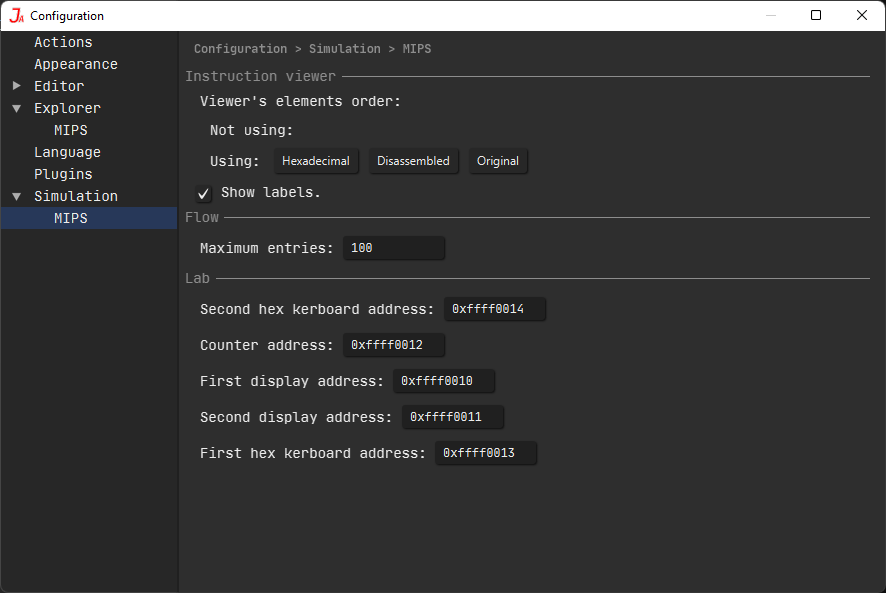
\includegraphics[width=0.8\textwidth]{images/base/jams-config}
    \caption{\textit{Interfaz de configuración}}
    \label{fig:jams-configuracion}
\end{figure}

\noindent Esta interfaz aprovecha los metadatos proporcionados por el archivo
de estructura para proporcionar una interacción adecuada entre el usuario
y los diferentes parámetros.
Esta interfaz es extensible, pudiendo los componentes añadir nuevos tipos de datos
proporcionando un \textbf{ValueEditor} y un \textbf{ValueConverter}.
Un \textbf{ValueConverter} permite transformar un objeto compuesto a una cadena
de caracteres y vice-versa.
Un \textbf{ValueEditor} proporciona una interfaz de edición adecuada para un
objeto compuesto.

\subsection{Secciones especiales}\label{subsec:secciones-especiales}

La interfaz de la configuración permite que ciertas gestiones se
gestionen de manera externa por un controlador diferente al de
por defecto.
Este es el caso de las secciones \textbf{Acciones} y \textbf{Plugins}.
Estas secciones tienen una estructura totalmente diferente a la
del resto de secciones, lo que permite al usuario modificar
de manera más eficiente sus parámetros.

\begin{figure}[H]
    \centering
    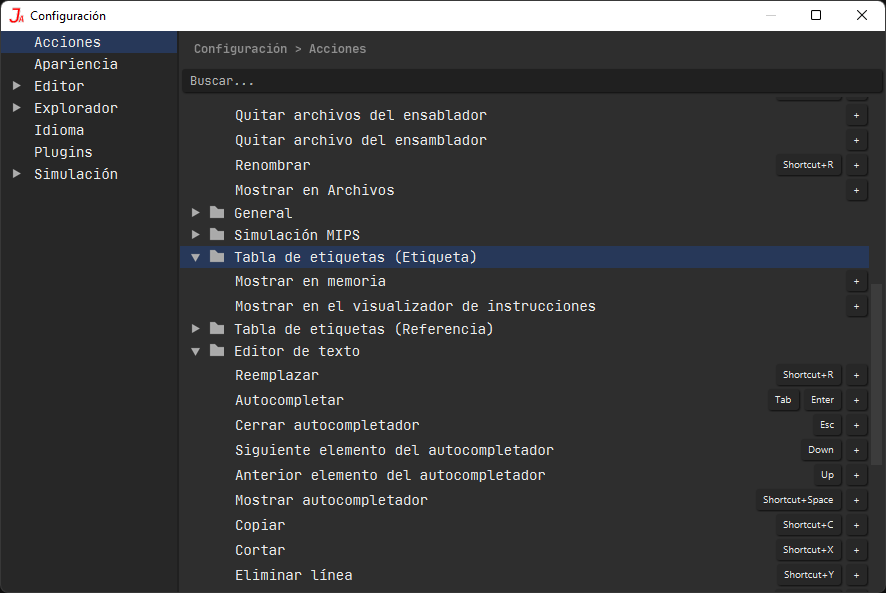
\includegraphics[width=0.8\textwidth]{images/base/jams-config-actions}
    \caption{\textit{Sección de acciones}}
    \label{fig:jams-configuracion-acciones}
\end{figure}


\section{Acciones}\label{sec:acciones}

Las acciones representan tareas que un usuario puede realizar de manera
\textbf{atómica}.
Las acciones pueden invocarse de diferentes maneras:
desde el menú principal, desde un menú de contexto
o usando una combinación de teclas modificable.
Cabe destacar que las acciones son \textbf{sensibles al contexto}:
una acción solo se podrá ejecutar en un determinado contexto
de la aplicación (el usuario no puede copiar un trozo de texto
en el explorador).

\noindent Los componentes pueden implementar nuevas acciones
creando una nueva clase que extienda \textbf{Action} o
\textbf{ContextAction}.
La clase \textbf{Action} es la clase básica para las acciones.
Las implementaciones deben implementar el funcionamiento
de la acción en el método \textbf{run}.
La clase \textbf{ContextAction} permite que la acción sea
mostrada en un menú contextual.
Las implementaciones de esta clase deben implementar
muchos más métodos que proporcionan información
sobre la viabilidad de la acción en diferentes contextos.


\section{Editor de texto}\label{sec:editor-de-texto}

El editor de texto es la tecnología que más iteraciones
ha sufrido en todo el desarrollo de \textit{JAMS},
siendo uno de los elementos más avanzados de toda
la aplicación.
El editor de texto presenta una arquitectura
\textbf{asíncrona}, y permite gestionar una gran
cantidad de líneas de texto sin bloquear la aplicación.

\subsection{Arquitectura}\label{subsec:arquitectura}

El editor de texto presenta una arquitectura
\textbf{Modelo-Vista-Controlador}:
\begin{itemize}
    \item \textbf{Vista:} la vista está gestionada
    por la librería \textit{RichTextFX}\cite{RICH_TEXT_FX}.
    \textit{RichTextFX} permite añadir estilos
    a secciones del texto.
    La vista está representada por la clase
    \textbf{CodeArea}.
    \item \textbf{Controlador:} el controlador está
    gestionado por la clase \textbf{CodeFileEditor}.
    Esta clase extiende \textbf{CodeArea}, y es la
    encargada de gestionar las entradas del usuario.
    \item \textbf{Modelo:} el modelo está representado
    por la clase \textbf{EditorIndex}.
    Las implementaciones de esta clase contienen
    una representación abstracta de los contenidos
    del editor de texto.
    El modelo se actualiza de manera asíncrona.
\end{itemize}

\subsection{Filosofía del modelo}\label{subsec:filosofía-del-modelo}

Debido a la gran complejidad de la arquitectura,
se ha definido una filosofía en el desarrollo
del modelo:
\begin{itemize}
    \item \textbf{Basado en elementos}: cada elemento representa
    un componente en el editor: un comentario, una instrucción,
    una etiqueta, etc.
    Los elementos son \textbf{casi inmutables}:
    solo sus inspecciones, alcances, y posición son mutables.
    \item Los elementos son recreados siempre que una línea
    es editada.
    \item Los elementos almacenan la mínima información
    posible.
    Esta información debe ser buscada usando los métodos
    de consulta proporcionados por el modelo.
    \item Los métodos de consult deben ser lo más rápidos
    posible.
    Las implementaciones por defecto utilizan la
    \textit{Stream API}\cite{STREAM_API} añadida en \textit{Java 8}.
\end{itemize}

\noindent \textbf{EditorIndexedElement} es la la interfaz principal
que representa un elemento.
Esta interfaz define los elementos de posición, tamaño, alcance,
jerarquía y contenido.
Los elementos concretos deben implementar esta interfaz.
Una implementación básica de un elemento puede encontrarse
en la clase \textbf{EditorIndexedElementImpl}.

\noindent Si un elemento desea ser referenciado, este debe
implementar la interfaz \textbf{EditorReferencedElement}.
Un elemento que implemente esta interfaz será gestionado
de manera diferente por el modelo.
De igual manera, si un elemento desea referenciar
otros elementos, este debe implementar la interfaz
\textbf{EditorReferencingElement}.
Estas dos interfaces no son incompatibles:
un elemento puede referenciar y ser referenciado
al mismo tiempo.

\noindent El modelo es un componente \textit{thread-safe}.
Para interactuar con él, un hilo debe reservar el acceso
al modelo y especificar si desea editar su estructura o
solo acceder a sus datos.
Si el hilo modifica el modelo, se creará dos evento de tipo
\textbf{IndexFinishEditEvent} y \textbf{IndexRequestRefreshEvent}
cuando termine la edición.

\subsection{Actualización del modelo}\label{subsec:actualizacion-del-modelo}

Cuando el controlador sigue el siguiente
protocolo cuando este recibe peticiones de modificación
por parte del usuario:
\begin{itemize}
    \item \textbf{Recolección:} las peticiones cercanas
    en el tiempo son registradas en una lista de peticiones.
    Esta lista es es procesada cuando el usuario deje
    de enviar modificaciones.
    \item \textbf{Compresión:} se descartan las peticiones
    de modificación que no van a tener efecto en el modelo.
    El caso más común de modificaciones sin efecto sería
    el de una cadena de modificaciones en una misma línea:
    solo el estado de la línea en la modificación final
    tendrá efecto en el modelo.
    \item \textbf{Actualización:} se genera una tarea
    asíncrona que modifica el modelo en base a las
    peticiones.
    \item \textbf{Finalización:} una vez el modelo
    es modificado, se envían una serie de eventos
    a la vista para que esta actualice el estilo
    de las líneas visibles.
\end{itemize}

\subsection{Estructura del modelo}\label{subsec:estructura-del-modelo}

El modelo presenta una arquitectura jerárquica de elementos:
un elemento tiene un padre y puede tener varios hijos.
Cada elemento contiene su posición inicial en el proyecto, la
longitud del texto y el texto representado.
Esta estructura puede considerarse una implementación de un
\textit{Rope}\cite{ROPES}, una estructura de dastos muy
utilizada para editores de texto.

\begin{center}
    \basictree{
        [Instruction 0 13 sw \$s0 0(\$s2)
        [Mnemonic 0 2 sw]
        [Parameter 3 3 \$s0
        [Register 3 3 \$s0]
        ]
        [Parameter 7 6 0(\$s2)
        [Immediate 7 1 0]
        [Register 9 3 \$s2]
        ]
        ]
    }
\end{center}

\noindent Los nodos hoja pueden implementar la interfaz
\textbf{EditorIndexStyleableElement}, permitiendo inyectar
estilos en la vista del editor de texto.
Esta interfaz solo presenta un método que pide una lista
de estilos.
\textit{JAMS} es el encargado de inyectar dichos estilos
en el editor cuando sea necesario.

\begin{figure}[H]
    \centering
    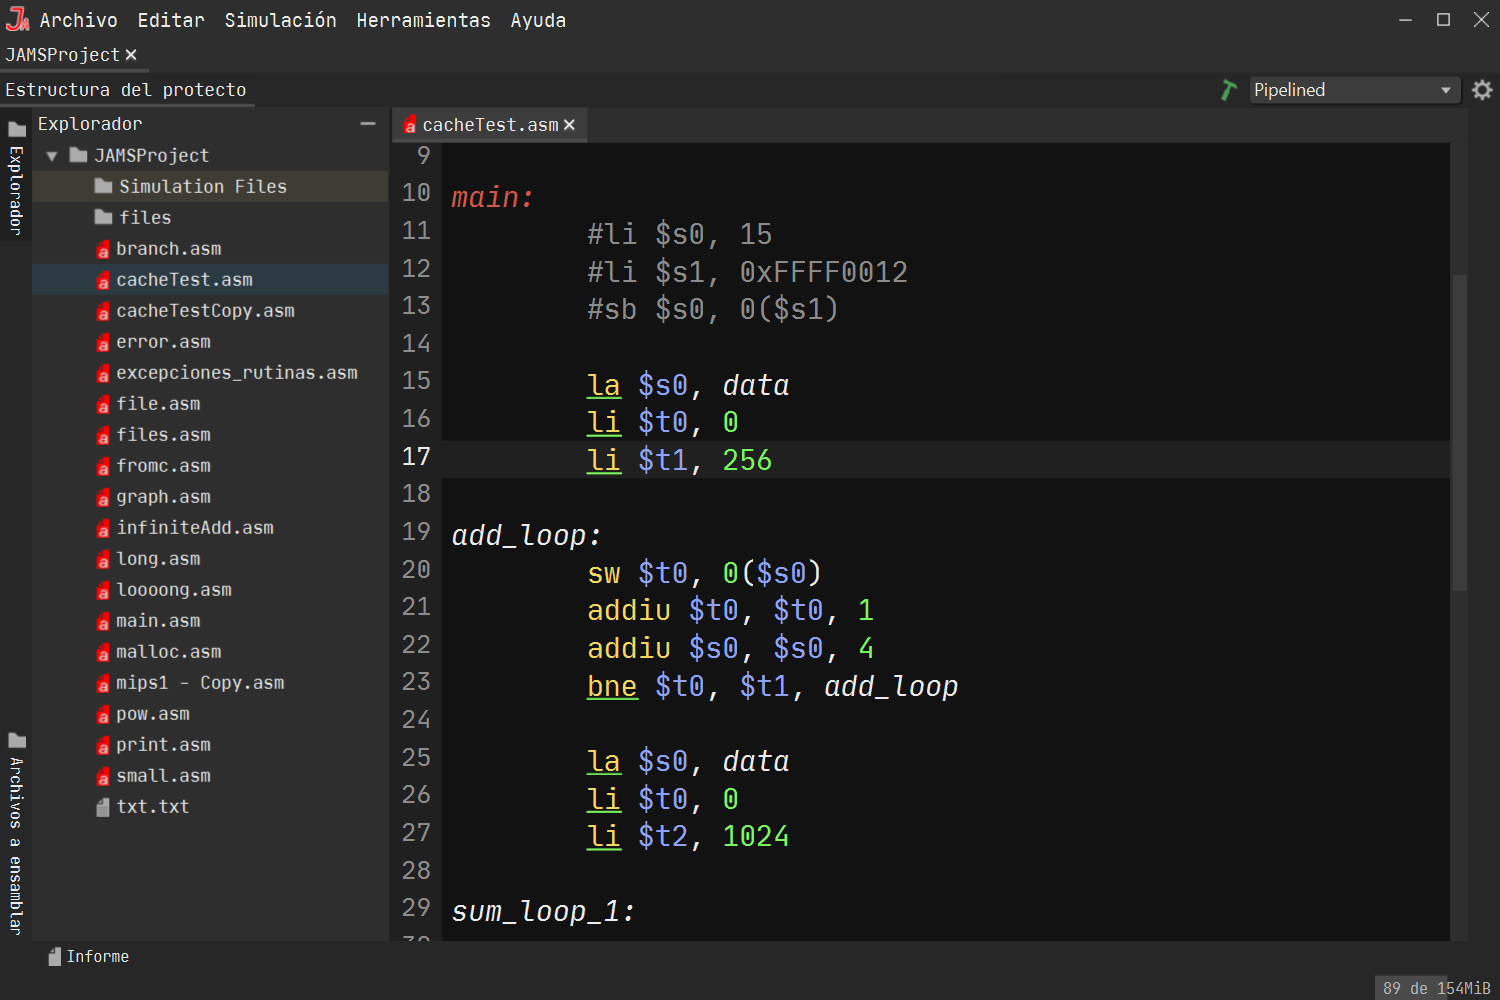
\includegraphics[width=0.8\textwidth]{images/base/jams-text-editor}
    \caption{Editor de texto con estilos inyectados}
    \label{fig:jams-editor-texto}
\end{figure}

\subsection{Referencias entre modelos}\label{subsec:referencias-entre-modelos}

Un modelo puede tener \textbf{referencias a elementos
presentes en otros modelos}.
Este es el caso de las etiquetas y macros globales.
La clase \textbf{ProjectGlobalIndex} permite la
comunicación entre modelos, actuando de intermediador.
Solo los elementos que están dentro de los archivos
de la lista de archivos a ensamblar serán tomados en cuenta.
Para evitar interbloqueos, todas las modificaciones
realizadas en un proyecto son gestionadas en el
mismo hilo.

\subsection{Implementaciones}\label{subsec:implementaciones}

\textit{JAMS} incorpora implementaciones básicas de los
diferentes componentes usados en el editor.
Una de las implementaciones más importantes es la que está
definida en la clase \textbf{EditorLineIndex}, la cual
implementa un modelo donde cada línea representa una
unidad autocontenida.

\noindent Otras implementaciones serían la de elementos
básicos y comunes en diferentes lenguajes ensamblador:
las etiquetas, las macros, las llamadas a macros o
los comentarios son ejemplos de elementos ya definidos.

\subsection{Autocompletación}\label{subsec:autocompletacion}

\textit{JAMS} aprovecha los datos proporcionados por
el modelo para implementar una interfaz de autocompletación
que el usuario puede usar en el editor.

\begin{figure}[H]
    \centering
    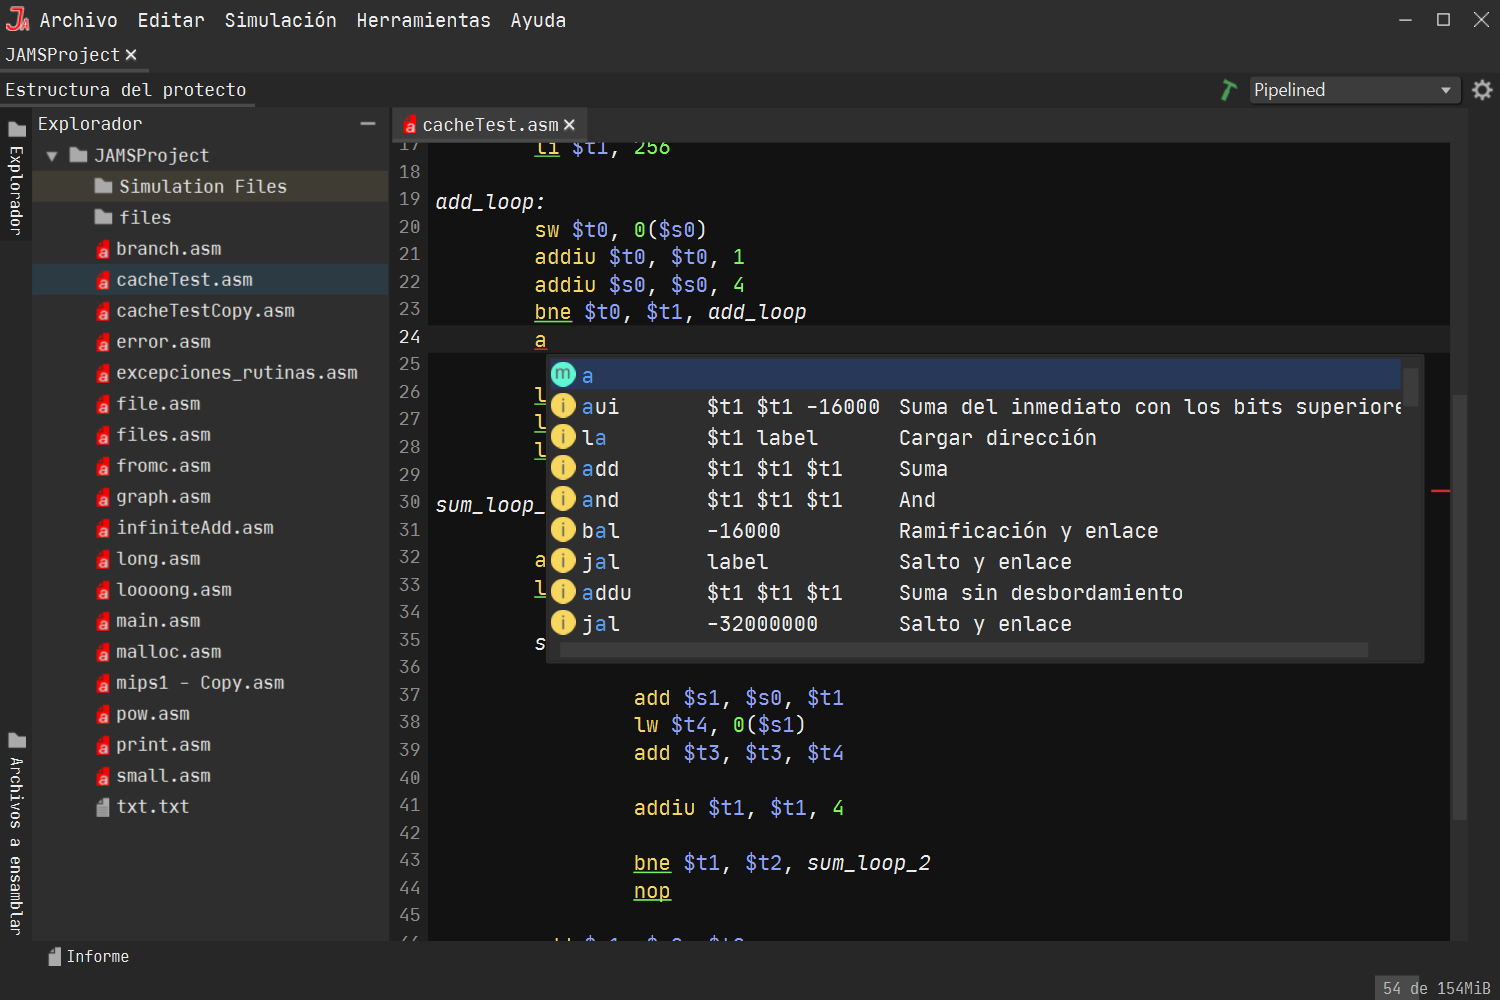
\includegraphics[width=0.8\textwidth]{images/base/jams-autocompletion}
    \caption{Autocompletador del editor de texto}
    \label{fig:jams-autocompletador}
\end{figure}

\noindent Igual que el propio editor de texto, esta interfaz
presenta una estructura modelo-vista-controlador:

\begin{itemize}
    \item \textbf{Controlador:} implementado en dos partes.
    \textit{JAMS} implementa las acciones de la interfaz,
    mientras que el desarrollador debe implementar el
    generador del modelo.
    \item \textbf{Modelo:} contiene los candidatos de
    la interfaz.
    \item \textbf{Vista:} implementa la interfaz que
    muestra los candidatos del modelo.
    \textit{JAMS} implementa una vista por defecto,
    pero los desarrolladores pueden implementar una
    vista propia.
\end{itemize}

\subsection{Documentación}\label{subsec:documentacion}

Como característica final, el editor de texto presenta
una interfaz de documentación que los proyectos
pueden utilizar para documentar sus diferentes
elementos.
Se puede acceder a la documentación con la secuencia por defecto
\textbf{Ctrl + Q}.

\begin{figure}[H]
    \centering
    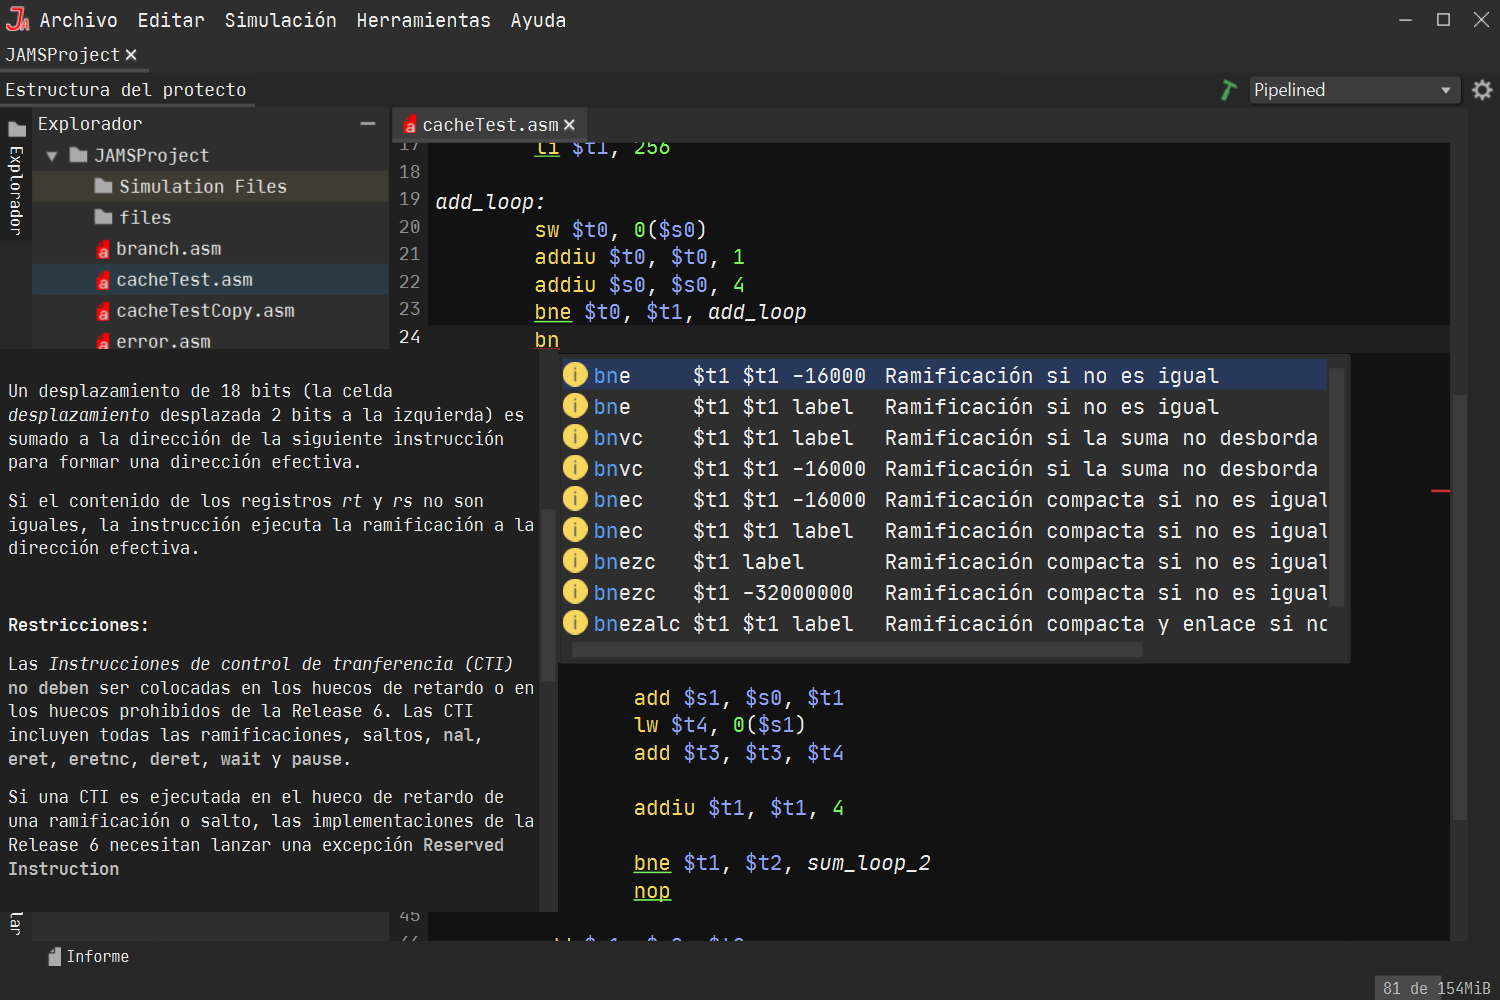
\includegraphics[width=0.8\textwidth]{images/base/jams-documentation}
    \caption{Documentación en el editor de texto}
    \label{fig:jams-documentacion}
\end{figure}